\chapter{MATERIALS AND METHODS}\label{methods}
\graphicspath{{images/}}

This section describes the components and methodology used in the development of the PRANK ankle rehabilitation robot, 
with reference to international standards that guide safety, performance, and software quality in rehabilitation robotics.

\section{Mechanical Structure}
The PRANK robot is designed with three degrees of freedom (DoF), enabling controlled movement in dorsiflexion/plantarflexion, inversion/eversion, and internal/external rotation. 
The mechanical structure follows safety principles outlined in ISO 13482 and ISO/TS 15066, which define requirements for personal care and collaborative robots. 
The frame is built using lightweight aluminum and 3D-printed joints to ensure modularity, ergonomic alignment, and safe physical interaction. 
The foot interface includes adjustable straps and a contoured support to minimize risk during use.

\section{Actuation and Sensing}
Each DoF is actuated by a brushless DC motor with integrated encoders, selected to meet performance criteria similar to those in ISO 9283. 
Torque estimation is achieved through current sensing and mechanical modeling. 
The system includes encoders for motion tracking and a 3D load cell for force feedback. 
Electrical safety considerations are guided by ISO 60601-1, addressing insulation, leakage current, and electromagnetic compatibility.

\section{Control Architecture}
The control system supports multiple rehabilitation modes: passive, assistive, and resistive. 
In assistive mode, the robot applies torque to guide the user’s movement along predefined trajectories. 
In resistive mode, it generates opposing torque to challenge the user’s effort and promote muscle strengthening. 
These modes are implemented using nonlinear control strategies and admitance-based control. 
The controller runs on a real-time embedded platform, with communication handled via serial or CAN protocols. 
Safety features include torque limits, emergency stop mechanisms, and compliance with ISO 10218-1 and ISO/TS 15066.

\section{Virtual Reality Interface}
A custom VR serious game developed in Unity provides interactive tasks that promote ankle mobility and coordination. 
The game receives real-time data from the robot and delivers visual, sound and haptic feedback to the user. 
Human-machine interaction principles from ISO 13482 and ISO/IEC 25010 are considered to ensure usability, engagement, and therapeutic relevance.

\section{Software Environment}
Software development follows lifecycle guidelines from ISO/IEC 62304 and ISO/IEC 12207, ensuring modularity, traceability, and maintainability. 
Embedded control is implemented in C++, while high-level coordination and data logging use C\# and Unity Game Engine. 
Control algorithms are validated in MATLAB/Simulink prior to deployment. Sensor data and user interaction metrics are logged for offline analysis and performance evaluation.

\section{Experimental Protocol (Planned)}
A pilot study will be conducted with healthy participants to evaluate system usability, comfort, and preliminary effectiveness. 
The protocol will include tasks in all three control modes and collect metrics such as range of motion, task completion time, and user feedback.
The ROM calculation will be verified using an optoelectronic tracking system. 

\section{System Architecture}
Figure \ref{fig:PRANK_schematic} presents the overall system architecture, detailing the integration between the embedded control 
hardware and the software modules responsible for data processing, user interaction, and rehabilitation logic. 

\begin{figure}
    \centering
    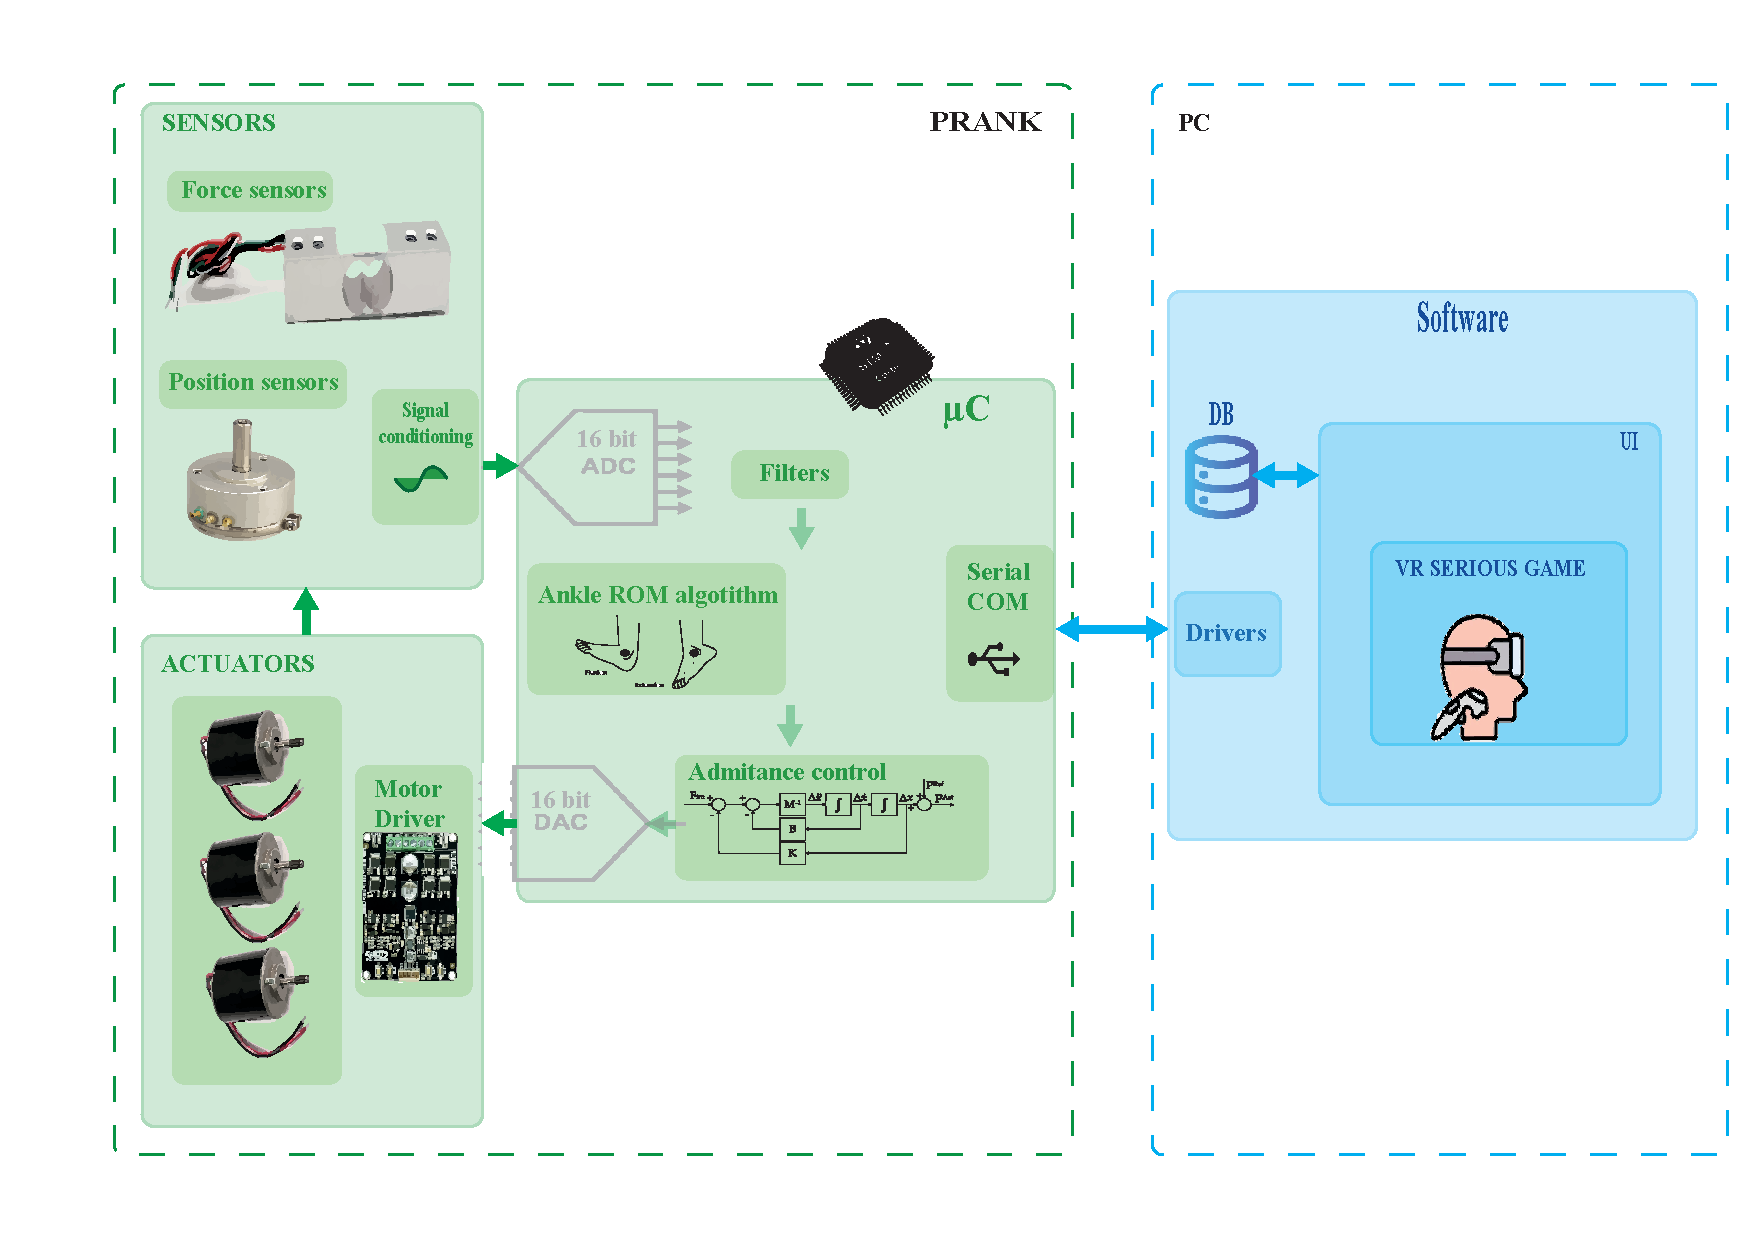
\includegraphics[width=1\textwidth]{PRANK-schematic.pdf}
    \caption{PRANK System schematic}
    \label{fig:PRANK_schematic}
\end{figure}